\section{Amplitude Formalism}
{\color{red}TODO: cite http://scipp.ucsc.edu/\textasciitilde haber/ph218/ExperimentersGuideToTheHelicityFormalism.pdf and S.U. Chung spin formalisms}
We begin by representing a single particle with four-momentum $\mathbf{P} = (E,\vec{p})$, spin $s$, and helicity $\lambda = -s, -s+1, \ldots, s-1, s$ with the notation $\ket{\vec{p},s,\lambda}$, a vector with Lorentz-invariant normalization
\begin{equation}
  \bra{\vec{p}',s',\lambda'}\ket{\vec{p},s,\lambda} = (2\pi)^3 2E \delta^3(\vec{p}'- \vec{p}) \delta_{s's}\delta{\lambda'\lambda}
\end{equation}

Since we are primarily interested in two-body decays, we can then represent a two-body state using the notation
\begin{equation}
  \ket{\vec{p}_1,s_1,\lambda_1} \otimes \ket{\vec{p}_2,s_2,\lambda_2} = \ket{\vec{p}_1,s_1,\lambda_1;\vec{p}_2,s_2,\lambda_2}
\end{equation}
with normalization
\begin{equation}\label{pwa:eq:two-particle-norm}
  \bra{\vec{p}'_1,s'_1,\lambda'_1;\vec{p}'_2,s'_2,\lambda'_2}\ket{\vec{p}_1,s_1,\lambda_1;\vec{p}_2,s_2,\lambda_2} = (2\pi)^6 4E_1 E_2 \delta^3(\vec{p}'_1 - \vec{p}_1)\delta^3(\vec{p}'_2 - \vec{p}_2)\delta_{s'_1 s_1}\delta_{s'_2 s_2}\delta_{\lambda'_1\lambda_1}\delta_{\lambda'_2\lambda_2}
\end{equation}

For simplification, we will work in the center-of-momentum frame. This allows us to use a single momentum, $\vec{p}_{1} = -\vec{p}_{2}$ without loss of generality in this frame. We can also assume that the spin of each particle is fixed and suppress $s_1$ and $s_2$ in the following derivations.

Next, we write the three-momentum in terms of spherical angles $\Omega_1 = (\theta_1, \varphi_1)$: $\vec{p}_1 = p_1(\sin\theta_1\cos\varphi_1, \sin\theta_1\sin\varphi_1, \cos\theta_1)$ where we use the shorthand $p_1\equiv\abs{\vec{p}_1}$. The equivalent coordinate transform must now be done on the normalization. It can be shown that,
\begin{align}
  \dd[3]{\vec{p}_1}\dd[3]{\vec{p}_2} &= \dd[3]{\vec{p}}\dd[3]{\vec{p_1}} \notag\\
                                     &= \dd[3]{\vec{p}}p_1^2 \dd{\left(p_1\right)}\dd[2]\Omega_1
\end{align}
where $\mathbf{P} = (E,\vec{p})$ is the total four-momentum in the center-of-momentum frame. Now note that, because we are in this frame, we can write $E = E_1 + E_2 = \sqrt{p_1^2 + m_1^2} + \sqrt{p_1^2 + m_2^2}$. Equivalently, we can write the differential element, $\dd{E}$, as
\begin{equation}
  \dd{E} = p_1\dd{p_1}\left(\frac{1}{\sqrt{p_1 + m_1^2}} + \frac{1}{\sqrt{p_1 + m_2^2}}\right) = p_1\dd{p_1}\left(\frac{1}{E_1} + \frac{1}{E_2}\right) = \frac{\sqrt{s}}{E_1E_2}p_1\dd{p_1}
\end{equation}

where $s = E^2$ is the Mandelstam variable, so
\begin{equation}
  \dd[3]{\vec{p}_1}\dd[3]{\vec{p}_2} = \dd[3]{\vec{p}}\dd{E}\frac{p_1E_1E_2}{\sqrt{s}}\dd[2]\Omega_1 = \frac{p_1E_1E_2}{\sqrt{s}}\dd[4]\mathbf{P}\dd[2]\Omega_1
\end{equation}

We can now take an arbitrary state and integrate over both sides:

\begin{align}
  \int\dd[3]{\vec{p}_1}\dd[3]{\vec{p}_2}\bra{\vec{p}'_1,\lambda'_1;\vec{p}'_2,\lambda'_2}\ket{\vec{p}_1,\lambda_1;\vec{p}2\lambda_2} &= \int\frac{p_1E_1E_2}{\sqrt{s}}\dd[4]\mathbf{P}\dd[2]\Omega_1\bra{p'_1,\Omega'_1,\lambda'_1,\lambda'_2}\ket{p_1,\Omega_1,\lambda_1,\lambda_2} \notag \\
  (2\pi)^6 4E_1E_2\delta_{\lambda'_1\lambda_1}\delta_{\lambda'_2\lambda_2} &= \int\frac{p_1E_1E_2}{\sqrt{s}}\dd[4]\mathbf{P}\dd[2]\Omega_1\bra{p'_1,\Omega'_1,\lambda'_1,\lambda'_2}\ket{p_1,\Omega_1,\lambda_1,\lambda_2} \notag \\
  (2\pi)^6 \frac{4\sqrt{s}}{p_1}\delta_{\lambda'_1\lambda_1}\delta_{\lambda'_2\lambda_2} &= \int\dd[4]\mathbf{P}\dd[2]\Omega_1\bra{p'_1,\Omega'_1,\lambda'_1,\lambda'_2}\ket{p_1,\Omega_1,\lambda_1,\lambda_2}\\
\end{align}

from \Cref{pwa:eq:two-particle-norm}, so the normalization factor should then be

\begin{equation}
  \bra{p'_1,\Omega'_1,\lambda'_1,\lambda'_2}\ket{p_1,\Omega_1,\lambda_1,\lambda_2} = (2\pi)^6\frac{4\sqrt{s}}{p_1}\delta^4(\mathbf{P}' - \mathbf{P})\delta^2(\Omega'_1 - \Omega_1)\delta_{\lambda'_1\lambda_1}\delta_{\lambda'_2\lambda_2}
\end{equation}

Since $\vec{p} = \vec{0}$ in the center-of-momentum frame, these states are eigenstates of the total four-momentum operator $\hat{\mathbf{P}}$, and we can factor it out as

\begin{equation}\label{pwa:eq:two-particle-state}
  \ket{p_1,\Omega_1,\lambda_1,\lambda_2} = (2\pi)^3\sqrt{\frac{4\sqrt{s}}{p_1}}\ket{\Omega_1,\lambda_1,\lambda_2}\ket{\mathbf{P}}
\end{equation}

We can then imagine replacing the two-body system with a single decaying particle. Such a particle can be defined in terms of its total angular momentum, $J$, and the eigenvalue of $\hat{J}_z$, $M$. Such a basis is an eigenstate of $\hat{J}^2$ and therefore transforms under rotations as

\begin{equation}\label{pwa:eq:jm-transform}
  \ket{p_1,J,M,\lambda_1,\lambda_2} \xrightarrow{R(\alpha,\beta,\gamma)} \sum_{M'} D^J_{M'M}(\alpha,\beta,\gamma)\ket{p_1,J,M',\lambda_1,\lambda_2}
\end{equation}

where $D^J_{M'M}(\alpha,\beta,\gamma)$ is the Wigner D-matrix with Euler angles $\alpha$, $\beta$, and $\gamma$. Next, we can define the transformation between our two-particle state and the single-particle state:

\begin{align}
  \ket{p_1,\Omega_1,\lambda_1,\lambda_2} &= \sum_{JM} c_{JM}\left(p_1,\Omega_1,\lambda_1,\lambda_2\right) \ket{p_1,J,M,\lambda_1,\lambda_2} \notag \\
  \ket{p_1,(0,0),\lambda_1,\lambda_2} &= \sum_{J} c_{J\lambda}\left(p_1,(0,0),\lambda_1,\lambda_2\right) \ket{p_1,J,\lambda,\lambda_1,\lambda_2}
\end{align}

where $\lambda = \lambda_1 - \lambda_2$ is the eigenvalue of $\hat{J}_z$ for the state where $\theta_1=\phi_1=0$, or $\vec{p}_1 = p_1\hat{z} = -\vec{p}_2$. To rotate from this specific choice back to an arbitrary $\Omega_1$, we apply a rotation $R(\varphi_1,\theta_1,-\varphi_1)$ according to \Cref{pwa:eq:jm-transform}:

\begin{align}
  \ket{p_1,\Omega_1,\lambda_1,\lambda_2} &= \sum_{J\lambda} c_{J\lambda}\left(p_1,(0,0),\lambda_1,\lambda_2\right)D^J_{M'\lambda}(\varphi_1,\theta_1,-\varphi_1)\ket{p_1,J,M',\lambda_1,\lambda_2} \\
  \sum_{JM} c_{JM}\left(p_1,\Omega_1,\lambda_1,\lambda_2\right)\ket{p_1,J,M',\lambda_1,\lambda_2} &= \sum_{J\lambda} c_{J\lambda}\left(p_1,(0,0),\lambda_1,\lambda_2\right)D^J_{M'\lambda}(\varphi_1,\theta_1,-\varphi_1)\ket{p_1,J,M',\lambda_1,\lambda_2}
\end{align}

so

\begin{equation}
  c_{JM}(p_1,\Omega_1,\lambda_1,\lambda_2) = c_{J\lambda}(p_1,(0,0),\lambda_1,\lambda_2)D^J_{M\lambda}(\varphi_1,\theta_1,-\varphi_1)
\end{equation}

By the Schur orthagonality relations applied to the Wigner D-matrices, we find that, without loss of generality,

\begin{equation}
  c_{JM} = c_J = \sqrt{\frac{2J + 1}{4\pi}}
\end{equation}

so that

\begin{equation}\label{pwa:eq:two-to-one}
  \ket{p_1,\Omega_1,\lambda_1,\lambda_2} = \sum_{JM}\sqrt{\frac{2J + 1}{4\pi}}D^J_{M\lambda}(\varphi_1,\theta_1,-\varphi_1)\ket{p_1,J,M,\lambda_1,\lambda_2}
\end{equation}

or

\begin{equation}\label{pwa:eq:jm-integral-form}
  \ket{p_1,J,M,\lambda_1,\lambda_2} = \sqrt{\frac{2J+1}{4\pi}}\int\dd{\Omega_1} D^{J*}_{M\lambda}(\varphi_1,\theta_1,-\varphi_1)\ket{p_1,\Omega_1,\lambda_1,\lambda_2}
\end{equation}

From this, it can also be shown that

\begin{equation}\label{pwa:eq:jm-two-particle-inner-product}
  \bra{J,M,\lambda'_1,\lambda'_2}\ket{\Omega_1,\lambda_1,\lambda_2} = \delta_{\lambda'_1\lambda_1}\delta_{\lambda'_2\lambda_2}\sqrt{\frac{2J + 1}{4\pi}} D^J_{M\lambda}(\varphi_1,\theta_1,-\varphi_1)
\end{equation}

Finally, these states are also eigenstates of $\hat{\mathbf{P}}$ since we are still working in the frame where $\vec{p} = \vec{0}$:

\begin{equation}\label{pwa:eq:one-particle-state}
  \ket{p_1,J,M,\lambda_1,\lambda_2} = (2\pi)^3\sqrt{\frac{4\sqrt{s}}{p_1}}\ket{J,M,\lambda_1,\lambda_2}\ket{\mathbf{P}}
\end{equation}

\subsection{Two-to-Two Scattering}
Let us now apply this to a two-to-two scattering problem $a + b \to c + d$ (which we will later apply to $\gamma p \to Xp$). We can write the initial and final states, working in the center-of-momentum frame, according to \Cref{pwa:eq:two-particle-state}. We will choose an initial frame where $\vec{p}_a \equiv p_i\hat{z} = -\vec{p}_b$. By definition, the final state momentum can also be defined relative to either particle, so we can choose $\vec{p}_f \equiv \vec{p}_c = -\vec{p}_d$:

\begin{align}
  \ket{i} &= (2\pi)^3\sqrt{\frac{4\sqrt{s}}{p_i}}\ket{(0,0),\lambda_a,\lambda_b}\ket{\mathbf{P_i}} \\
  \ket{f} &= (2\pi)^3\sqrt{\frac{4\sqrt{s}}{p_f}}\ket{\Omega_f,\lambda_a,\lambda_b}\ket{\mathbf{P_f}}
\end{align}

We can define a scattering amplitude between state $\ket{i}$ and $\ket{j}$ as $S$ such that

\begin{align}\label{pwa:eq:scattering-amplitude-def}
  \mel{f}{S}{i} &= (2\pi)^6 \sqrt{\frac{16 s}{p_i p_f}}\bra{\mathbf{P}_f}\mel{\Omega_f,\lambda_c,\lambda_d}{S}{(0,0),\lambda_a,\lambda_b}\ket{\mathbf{P}_i} \notag \\
                &= (2\pi)^6 \bra{\mathbf{P}_f}\ket{\mathbf{P}_i} \sqrt{\frac{16 s}{p_i p_f}}\mel{\Omega_f,\lambda_c,\lambda_d}{S(s)}{(0,0),\lambda_a,\lambda_b} \notag \\
                &= (2\pi)^6 \delta^4\left(\mathbf{P}_f - \mathbf{P}_i\right) \sqrt{\frac{16 s}{p_i p_f}}\mel{\Omega_f,\lambda_c,\lambda_d}{S(s)}{(0,0),\lambda_a,\lambda_b}
\end{align}

Since we mostly do not care about the case where the initial and final states are the same, we will define (by convention) a transition amplitude which factors out such scatterings:

\begin{equation}
  S_{fi} = \delta_{fi} + \imath (2\pi)^4 \delta^4(\mathbf{P}_f - \mathbf{P}_i) T_{fi}
\end{equation}

such that

\begin{equation}
  \mel{f}{T}{i} = -\imath(2\pi)^2\sqrt{\frac{16s}{p_fp_i}}\mel{\Omega_f,\lambda_c,\lambda_d}{T(s)}{(0,0),\lambda_a,\lambda_b}
\end{equation}

By inserting a complete set of states for both the initial and final two-particle systems:

{\color{red}TODO: Fix box}
\begin{equation}
  \mel{f}{T}{i} = -\imath(2\pi)^2\sqrt{\frac{16s}{p_fp_i}}\bra{\Omega_f,\lambda_f,\lambda_d}\left(\sum_{JM}\ket{J,M,\lambda_c,\lambda_d}\bra{J,M,\lambda_c,\lambda_d}\right) T(s) \left(\sum_{J'M'}\ket{J',M',\lambda_a,\lambda_b}\bra{J',M',\lambda_a,\lambda_b}\right)\ket{(0,0),\lambda_a,\lambda_b}
\end{equation}

From \Cref{pwa:eq:two-to-one}, we can write this as

\begin{align}\label{pwa:eq:scattering-mel}
  \mel{f}{T}{i} &= -\imath(2\pi)^2\sqrt{\frac{16s}{p_fp_i}}\sum_{JMJ'M'}\sqrt{\frac{2J+1}{4\pi}}\sqrt{\frac{2J'+1}{4\pi}}D^{J*}_{M\lambda_f}(\varphi_f,\theta_f,-\varphi_f)\mel{J,M,\lambda_c,\lambda_d}{T(s)}{J',M',\lambda_a,\lambda_b} D^{J'}_{M'\lambda_f}(0,0,0) \notag \\
                &= -\imath(2\pi)^2\sqrt{\frac{16s}{p_fp_i}}\sum_{JMJ'M'}\sqrt{\frac{2J+1}{4\pi}}\sqrt{\frac{2J'+1}{4\pi}}D^{J*}_{M\lambda_f}(\varphi_f,\theta_f,-\varphi_f)\delta_{JJ'}\delta_{MM'}\mel{\lambda_c,\lambda_d}{T^J(s)}{\lambda_a,\lambda_b} D^{J'}_{M'\lambda_f}(0,0,0) \notag \\
                &= -\imath(2\pi)^2\sqrt{\frac{16s}{p_fp_i}} \sum_{J} \left(\frac{2J + 1}{4\pi}\right) D^{J*}_{\lambda_i\lambda_f}(\varphi_f,\theta_f,-\varphi_f)\mel{\lambda_c,\lambda_d}{T^J(s)}{\lambda_a,\lambda_b}
\end{align}

where $\lambda_i \equiv \lambda_a - \lambda_b$ and $\lambda_f \equiv \lambda_c - \lambda_d$. The Wigner D-matrix is related to Wigner's small d-matrix by

\begin{equation}
  D^{j*}_{m'm}(\alpha,\beta,\gamma)\equiv e^{\imath m'\alpha}d^j_{m'm}(\beta)e^{\imath m \gamma}
\end{equation}

so we can also write

\begin{align}\label{pwa:eq:scattering-mel2}
  \mel{f}{T}{i} &= -\imath(2\pi)^2\sqrt{\frac{16s}{p_fp_i}} \sum_J \left(\frac{2J + 1}{4\pi}\right) e^{-\imath(\lambda_f - \lambda_i)\varphi_f}d^J_{\lambda_i\lambda_j}(\theta_f) \mel{\lambda_c,\lambda_d}{T^J(s)}{\lambda_a,\lambda_b} \notag \\
                &= -\imath(2\pi)^2\sqrt{\frac{16s}{p_fp_i}} \sum_J \left(\frac{2J + 1}{4\pi}\right) e^{-\imath(\lambda_f - \lambda_i)\varphi_f}d^J_{\lambda_i\lambda_j}(\theta_f) T^{J}_{\lambda_c,\lambda_d;\lambda_a,\lambda_b}(s) \notag \\
                &= (-\imath)4\pi\sqrt{\frac{s}{p_fp_i}} \sum_J \left(2J + 1\right) e^{-\imath(\lambda_f - \lambda_i)\varphi_f}d^J_{\lambda_i\lambda_j}(\theta_f) T^{J}_{\lambda_c,\lambda_d;\lambda_a,\lambda_b}(s)
\end{align}

The actual observable we care about is the differential cross section,

\begin{equation}\label{pwa:eq:scattering-xsection}
  \pdv{\sigma}{s}{\Omega_f} \propto \abs{\mel{f}{T}{i}}^2
\end{equation}

so we can ignore the overall factor of $-\imath$ in \Cref{pwa:eq:scattering-mel,pwa:eq:scattering-mel2}.

\subsection{Two-Body Decays}

Next, we will give a similar treatment to a particle $d \to 1 + 2$ where $X$ is a particle with mass $m_X$, spin $J_X$, and spin projection $M_X$. Again, we will work in the center-of-momentum frame of this decay, so we can chose $\vec{p}_f \equiv \vec{p}_1 = -\vec{p}_2$. In the rest frame of particle $X$, we get the relation $s_X \equiv E_X^2 = m_X^2$ From \Cref{pwa:eq:two-particle-state}, we write the final state as

\begin{equation}
  \ket{f} = (2\pi)^3\sqrt{\frac{4m_X}{p_f}}\ket{\Omega_f,\lambda_1,\lambda_2}\ket{\mathbf{P}_f}
\end{equation}

while the initial state has no dependence on the final state helicities and is given by

\begin{equation}
  \ket{i} = \ket{J,M}\ket{\mathbf{P}_X}
\end{equation}

Given a decay amplitude $A$ which functions like our scattering matrix $S$ in \Cref{pwa:eq:scattering-amplitude-def}, we can write

\begin{align}
  \mel{f}{A}{i} &= (2\pi)^3\sqrt{\frac{4m_X}{p_f}}\mel{\Omega_f,\lambda_1,\lambda_2}{A}{J_X,M_X} \notag \\
                &= (2\pi)^3\sqrt{\frac{4m_X}{p_f}}\bra{\Omega_f,\lambda_1,\lambda_2}\left(\sum_{J'M'}\ket{J',M',\lambda_1,\lambda_2}\bra{J',M',\lambda_1,\lambda_2}\right)A\ket{J_X,M_X} \notag \\
                &= (2\pi)^3 \sqrt{\frac{4m_X}{p_f}}\sum_{J'M'}\sqrt{\frac{2J'+1}{4\pi}}D^{J'*}_{M'\lambda}(\varphi_f,\theta_f,-\varphi_f)\mel{J',M',\lambda_1,\lambda_2}{A}{J_X,M_X}
\end{align}

where the last line comes from \Cref{pwa:eq:jm-two-particle-inner-product}. Since $\bra{J',M'}\ket{J_X,M_X} = \delta_{J'J_X}\delta_{M'M_X}$, (see \Cref{pwa:eq:jm-integral-form}), and because the matrix element should be rotationally invariant, we can write $\mel{J',M',\lambda_1,\lambda_2}{A}{J_X,M_X} \equiv \delta_{J'J_X}\delta_{M'M_X} A_{\lambda_1\lambda_2}$:

\begin{equation}\label{pwa:eq:decay-mel}
  \mel{f}{A}{i} = (2\pi)^3\sqrt{\frac{4m_X}{p_f}}\sqrt{\frac{2J_X+1}{4\pi}}D^{J_X*}_{M_X\lambda}(\varphi_f,\theta_f,-\varphi_f) A_{\lambda_1\lambda_2}
\end{equation}

Again, to relate this to an actual experimental observable, we take the square of the norm. Because we don't actually measure the helicities $\lambda_1$ or $\lambda_2$ in the GlueX experiment, we can instead sum over them:

\begin{equation}\label{pwa:eq:decay-xsection}
  \pdv{\sigma}{\Omega_f} = \sum_{\lambda_1\lambda_2}(2\pi)^3\frac{2J_X+1}{\pi }\frac{m_X}{p_f}\abs{D^{J_X*}_{M_X\lambda}(\varphi_f,\theta_f,-\varphi_f)A_{\lambda_1\lambda_2}}^2
\end{equation}

\subsection{Production Amplitudes}
{\color{red}TODO: cite https://link.springer.com/article/10.1140/epjc/s10052-020-7930-x}
Now we are ready to put everything together to work out a cross section for the reaction $\gamma + p \to [X \to K_S + K_S] + p'$. This is somewhat equivalent to combining \Cref{pwa:eq:scattering-mel} and \Cref{pwa:eq:decay-mel}, but the decay amplitude now includes the state of the spectator (recoil) proton. To temporarily maintain similar notation, we can write this reaction as $a + b \to c + X$ where $X \to 1 + 2$. We can write the matrix element as

\section{Second attempt}
{\color{red}Following https://onlinelibrary.wiley.com/doi/10.1155/2020/6674595}
% \begin{figure}[h]
%   \centering
%   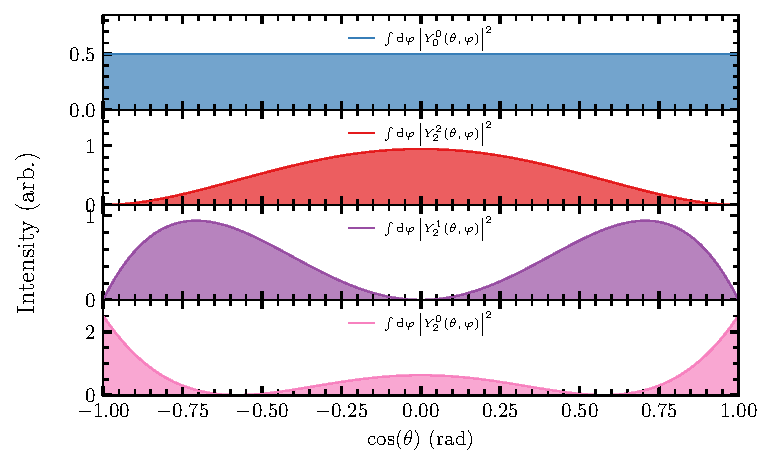
\includegraphics[width=.8\columnwidth]{spherical_harmonics}
%   \label{fig:sph_harm}
%   \caption{Absolute square of spherical harmonics for S- and D-waves integrated over $\varphi$.}
% \end{figure}
% \begin{figure}[h]
%   \centering
%   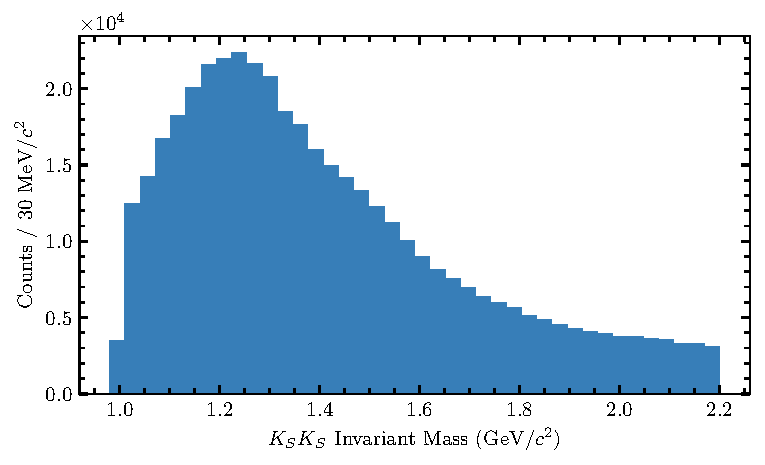
\includegraphics[width=.8\columnwidth]{KsKs_Inv_Mass_S17_fiducial}
%   \label{fig:mass_all_fiducial}
%   \caption{Absolute square of spherical harmonics for S- and D-waves integrated over $\varphi$.}
% \end{figure}


\subsection{Including Linear Polarization}
\section{The $Z_\ell^m$ Amplitude}
\section{The $K$-Matrix Parameterization}
\section{Waveset Selection}
